\section{Gustavo}

\setbeamertemplate{caption}{\raggedright\insertcaption\par}
\begin{frame}{Introduction}{Gustavo S. Buschle\newline<gbusch14@student.aau.dk>}
    \begin{figure}[h!]
        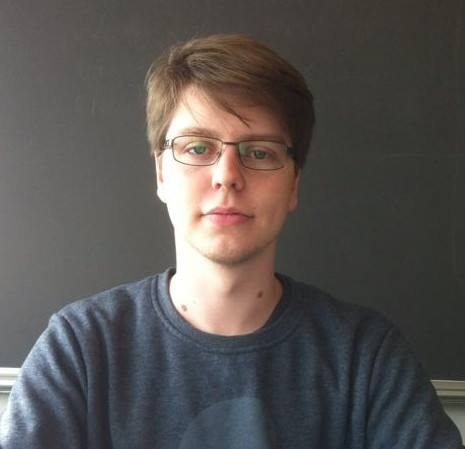
\includegraphics[width=0.3\textwidth]{images/gustavo.jpg}
        \caption{Gustavo S. Buschle}
        \centering
    \end{figure}
\end{frame}
\setbeamertemplate{caption}[default]

\begin{frame}{The Lidar}{Gustavo S. Buschle\newline<gbusch14@student.aau.dk>}
    \begin{itemize}
        \item <1-> Assembly of Parts
            \begin{itemize}
                \item <2-> I2C to talk to laser
                \item <3-> 3D printed case (Not very well)
            \end{itemize}
        \item <4-> Two versions of the lidar
        \begin{itemize}
            \item <5-> V1: Arduino drives stepper and Pi talks to laser
                \begin{itemize}
                    \item <6-> Fragmented development
                    \item <7-> Hard to sync
                \end{itemize}
            \item <8-> V2: Arduino only used for power 
                \begin{itemize}
                    \item <9-> Slow
                \end{itemize}
        \end{itemize}
    \end{itemize}
        \begin{figure}[h!]
            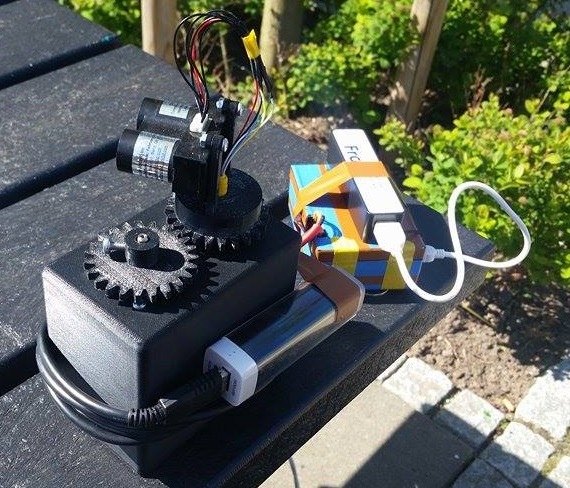
\includegraphics[width=0.3\textwidth]{images/lidarpi.jpg}
        \end{figure}
\end{frame}

\begin{frame}{ROS}{Gustavo S. Buschle\newline<gbusch14@student.aau.dk>}
    \begin{itemize}
        \item <1-> Learning Curve
            \begin{itemize}
                \item <1-> We didn't understand how ROS worked until development.
                \item <2-> There were a lot of different configurations that we needed to change
            \end{itemize}
        \item <3-> ROS components we used
            \begin{itemize}
                \item <3-> HectoSLAM
                \item <4-> rviz
            \end{itemize}
    \end{itemize}
\end{frame}

\begin{frame}{SLAM}{Gustavo S. Buschle\newline<gbusch14@student.aau.dk>}
    \begin{itemize}
        \item <1-> We didn't actually use it completely
        \begin{figure}[h!]
            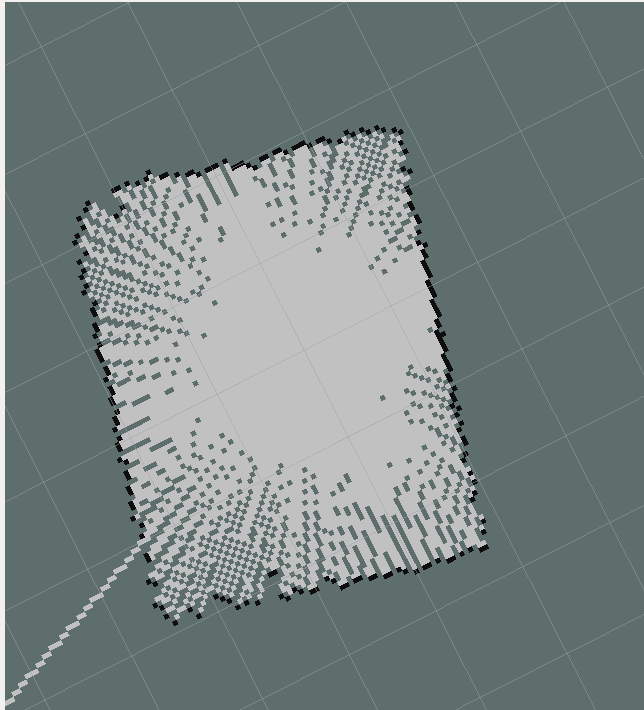
\includegraphics[width=0.3\textwidth]{images/hector.png}
        \end{figure}
        \item <2-> Linux time problems
    \end{itemize}
\end{frame}
